%\chapterimage{Water1.png} % Chapter heading image

%\chapter{Water Regulations}
%
%
%
%
%\chapterimage{AppendixChapterImage} % Chapter heading image
%\chapter*{Appendix}
%\thispagestyle{empty}
%\topskip0pt
%\vspace*{\fill}
%\begin{center}
%\textbf{Table of Contents - Drinking Water Regulations in California Code of Regulations}
%\end{center}
%\vspace*{\fill}
%\newpage
%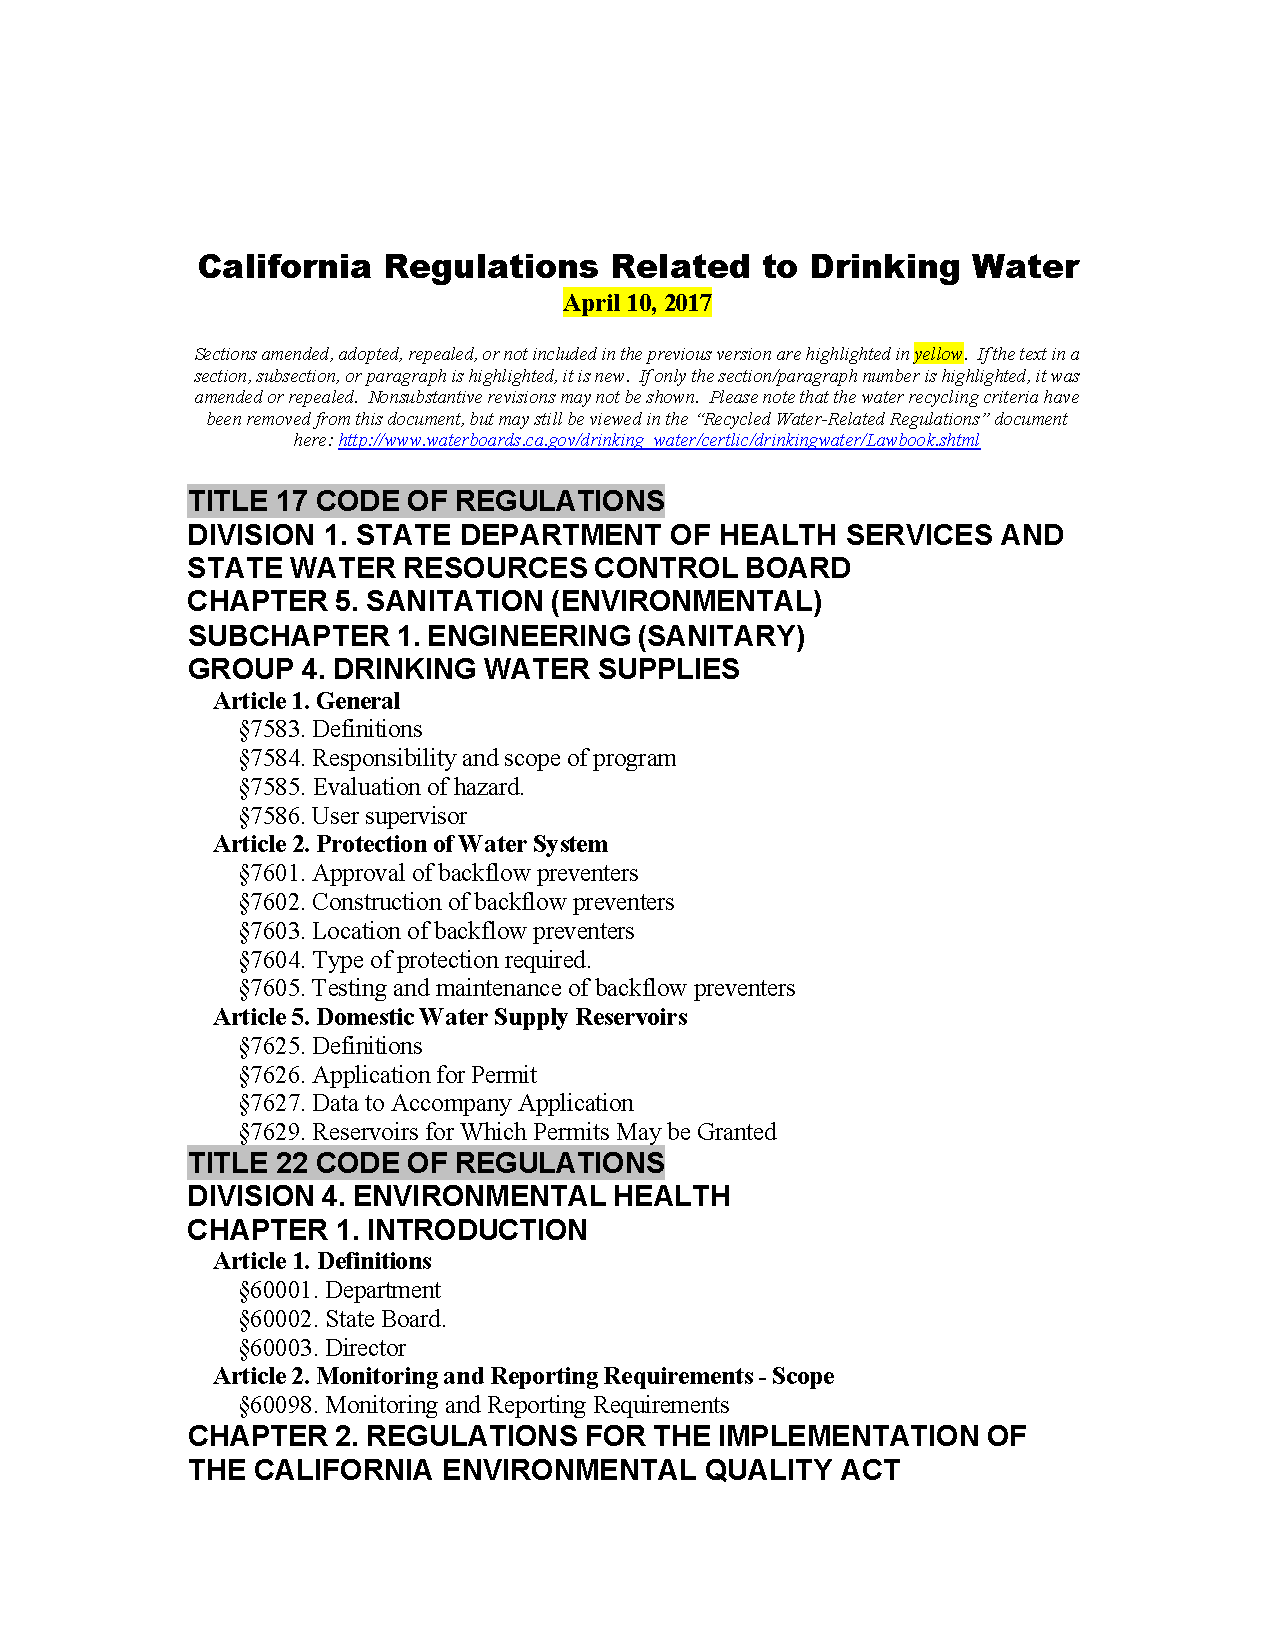
\includepdf[pages={1-12}]{CaliforniaDrinkingWaterRegulationsTOC}
%\newpage
%\thispagestyle{empty}
%\topskip0pt
%\vspace*{\fill}
%\begin{center}
%\textbf{American Water College - Water Treatment Operator Certification in California}
%\end{center}
%\vspace*{\fill}
%\newpage


%\newpage
%
%%\begin{dBox}
%%\lipsum*[1]
%%\end{dBox}
%
%
%% Please add the following required packages to your document preamble:
%% \usepackage{multirow}
%% \usepackage[table,xcdraw]{xcolor}
%% If you use beamer only pass "xcolor=table" option, i.e. \documentclass[xcolor=table]{beamer}
%\begin{table}[]
%\scriptsize
%\begin{tabular}{|p{2cm}|p{3cm}|p{3cm}|p{3cm}|}
%\hline
%\rowcolor[HTML]{1F15AD} 
%\multicolumn{1}{|c|}{\cellcolor[HTML]{1F15AD}{\color[HTML]{FFFFFF} Contaminant}} 
%
%& \multicolumn{1}{c|}{\cellcolor[HTML]{1F15AD}{\color[HTML]{FFFFFF} Maximum   Contaminant Level (MCL)}} 
%
%& \multicolumn{1}{c|}{\cellcolor[HTML]{1F15AD}{\color[HTML]{FFFFFF} Monitoring   Requirement – Surface Only or Combination}}                                                                                                                
%
%& \multicolumn{1}{c|}{\cellcolor[HTML]{1F15AD}{\color[HTML]{FFFFFF} Check Sampling,   Reporting and Public Notice}}                                                                                     \\ \hline
%                                                                                 & \textless{}40   samples/month, no more than 1 positive                                                &                                                                                                                                                                                                                                           & Repeat samples   are required for each coliform- positive sample. All samples must be   collected the same day.                                                                                       \\ \cline{2-2} \cline{4-4} 
%                                                                                 & \textgreater{}40 samples/month, no more than 5\%   positive.                                          &                                                                                                                                                                                                                                           & At least one   sample from same tap as original, another from an up- stream connection, and   one from downstream. All coliform positives must be tested for presence of   fecal coliform or E.coli.  \\ \cline{2-2} \cline{4-4} 
%
%
%\multirow{-3}{*}{Total coliform}                                                 &                                                                                                       
%
%& \multirow{-3}{*}{Compliance is based on  the presence or absence of total coliforms. All coliform positives must be   tested for presence of fecal coliform or E.coli. The total number of samples is based on the population   served.} & If repeat   sample is fecal coliform positive or if the original fecal coliform or E.coli   positive is followed by a total coliform positive, the state must be notified   on the same business day. \\ \hline
%                                                                                
%                                                                                 &                                                                                                       
%                                                                                 &                                                                                                                                                                                                                                           
%                                                                                 & Failure to meet   total percent inactivation on more than two days in a month is a violation.                                                                                                         \\ \cline{4-4} 
%
%\multirow{-2}{*}{Giardia Lamblis}                                                
%
%& \multirow{-2}{*}{3-Log (99.9\%) removal   or inactivation.}                                           & \multirow{-2}{*}{Based on calculated   residual disinfectant CT values.}                                                                                                                                                                  & State must be notified within one business day when disinfectant   residual is less than 0.2 mg/L.                                                                                                    \\ \hline
%Viruses                                                                          & 4-Log (99.99\%)   removal or inactivation                                                             &                                                                                                                                                                                                                                           & If residual is   less than 0.2 mg/L, then sampling must be every 4 hours until residual is   restored.                                                                                                \\ \hline
%\end{tabular}
%\end{table}



%\chapterimage{QuizCover} % Chapter heading image

% \chapter*{Regulations}
% \newpage
% \textbf{Match the following:}\\
% \begin{table}[ht]
% \renewcommand{\arraystretch}{2.4}
% \scriptsize
% \begin{tabular}{p{5cm}}
% A. Information Collection Rule                       \\

% B.  Long Term 1-Enhanced Surface Water Treatment Rule \\

% C.  Ground Water                                      \\

% D.  Stage 2-Disinfectant Byproduct Rule               \\

% E. Long Term 2-Enhanced Surface Water Treatment Rule \\

% F. Interim Enhanced Surface Water Treatment Rule     \\

% G. Disinfection/Disinfection Byproduct Rule, Phase I \\

% H. Total Coliform Rule                               \\

% I. Surface Water Treatment Rule                      \\

% \end{tabular}
% \renewcommand{\arraystretch}{1.2}
% \begin{tabular}{p{9cm}}
% i.  This   rule provides guidelines for identifying ground water sources at risk for   contamination and guidelines for taking corrective action.                                                                                                                                                \\
% \hline 
% ii.  This rule primarily addresses the reduction of risk from Cryptosporidium by limiting the   turbidity levels of filter effluents.                                                                                                                                                             \\
% \hline 
% iii.  This rule requires all systems serving fewer than 10,000 people   to achieve at least 99\% removal or inactivation of Cryptosporidium.                                                                                                                                                       \\
% \hline 
% iv.  This rule sets the monitoring and compliance requirements for   coliform bacteria.                                                                                                                                                                                                           \\
% \hline 
% v.  It required large public water suppliers to undertake monitoring   of microbial and disinfection byproducts in their water systems.                                                                                                                                                          \\
% \hline 
% vi.  This rule set maximum contaminant level goals and maximum   contaminant levels for trihalomethanes, five haleocetic acids, bromate and   chlorite.                                                                                                                                           \\
% \hline 
% vii.  This rule required all surface waters or ground waters under the   influence of surface waters to provide filtration and/or disinfection of the   source to meet 3 log removal or inactivation of Giardia   Lamblia cysts and 4 log removal or inactivation of   enteric viruses.           \\
% \hline 
% viii.  This rule is anticipated to propose treatment techniques to   improve control of microbial pathogens, specifically including Cryptosporidium. The techniques are   to consider the risks of treatment for Cryptospodrium   versus the potential for generation of   disinfection byproducts. \\
% \hline 
% ix.  The purpose of this rule is to assess information and research   that was not fully considered in the Stage 1 process or that has only been   available since 1998, as it relates to microbial standards to protect public   health.                                                        \\
% \hline 
% \end{tabular}
% \end{table}
% \textbf{Answers:}\\
% \begin{enumerate}[A.]
% \item \rule{1cm}{.5pt}
% \vspace{0.2cm}
% \item \rule{1cm}{.5pt}
% \vspace{0.2cm}
% \item \rule{1cm}{.5pt}
% \vspace{0.2cm}
% \item \rule{1cm}{.5pt}
% \vspace{0.2cm}
% \item \rule{1cm}{.5pt}
% \vspace{0.2cm}
% \item \rule{1cm}{.5pt}
% \vspace{0.2cm}
% \item \rule{1cm}{.5pt}
% \vspace{0.2cm}
% \item \rule{1cm}{.5pt}
% \vspace{0.2cm}\\
% \item \rule{1cm}{.5pt}
% \vspace{0.2cm}\\
% \end{enumerate}

% \newpage
% \textbf{Multiple Choice:}\\
\begin{enumerate}

\item Primary drinking water standards are set to protect the public from illnesses as a direct result in drinking water that exceeds maximum set levels. Secondary standards were set to alert the public to\\
a. the incidences of local cancer numbers\\
b. dissolved solids in water\\
c. immediate health concerns\\
d. radiological conditions concerning drinking water\\
e. *aesthetic issues with drinking water\\
\item A positive fecal coliform test must be reported to the primacy agency within\\
a. 8 hours.\\
b. 12 hours.\\
c. 24 hours.\\
d. 48 hours.\\
\item Which agency sets legal limits on the concentration levels of harmful contaminants in potable water distributed to customers?\\
a. National Primary Drinking Water Regulations\\
b. United States Environmental Protection Agency\\
c. United States Public Health Service\\
d. Occupational Health and Safety Organization\\
\item Which may be substituted for the analysis of residual disinfectant concentration, when total coliforms are also sampled at the same sampling point?\\
a. Heterotrophic plate count (HPC)\\
b. Fecal coliforms\\
c. Giardia lamblia\\
d. Combined chlorine\\
\item What does the acronym MCL stand for?\\
a. Minimum contaminant level\\
b. Micron contaminant level\\
c. Maximum contaminant level\\
d. Milligrams counted last\\
\item How long do sanitary surveys have to be retained for records?\\
a. 3 years\\
b. 5 years\\
c. 7 years\\
d. 10 years\\
\item The most severe water system violation that requires the fastest public notification\\
a. Tier I\\
b. Tier II\\
c. Tier III\\
d. Tier IV 8. The primacy agency may grant a variance or exemption as long as\\
a. The agency is using the Best Available Technology\\
b. There is no threat to public health\\
c. There is never a scenario for a variance or exemption\\
d. Both A. and B.\\
\item A public water system that serves at least 25 people six months out of the year\\
a. Nontransient noncommunity\\
b. Transient noncommunity\\
c. Community public water system\\
d. None of the above\\
\item Regulations based on the aesthetic quality of drinking water\\
a. Primary Standards\\
b. Secondary Standards\\
c. Microbiological Standards\\
d. Radiological Standards\\
\item The lowest reportable limit for a water sample\\
a. $0.5 \mathrm{mg} / 1$\\
b. Zero\\
c. Public health goal\\
d. Detection Level for reporting\\
\item Primary Standards are based on\\
a. Color and Taste\\
b. Aesthetic quality\\
c. Public Health\\
d. Odor\\
\item A disease causing microorganism\\
a. Pathogen\\
b. Colilert\\
c. Pathological\\
d. Turbidity\\
\item According to Surface Water Treatment Rule, what is the combined inactivation and removal for Giardia?\\
a. $1.0 \log s$\\
b. $2.0 \log \mathrm{s}$\\
c. $3.0 \log s$\\
d. 4.0 Logs\\
\item What is the equivalency expressed as a percentage for the SWTR inactivation and removal of viruses?\\
a. $99.9 \%$\\
b. $99.99 \%$\\
c. $99.0 \%$\\
d. $99.999 \%$\\
\item A water agency that takes more than 40 coliform samples must fall under what percentile?\\
a. $10 \%$\\
b. $7 \%$\\
c. $5 \%$\\
d. No positive samples allowable\\
\item The National Primary Drinking Water Regulations apply to drinking water contaminants that may have adverse effects on\\
a. Water color\\
b. Water taste\\
c. Water odor\\
d. Human health\\
\item Which of the following is considered an acute risk to health?\\
a. Two Tier 2 violations\\
b. One Tier 2 violation\\
c. Two Tier 1 violations\\
d. One Tier 1 violation\\
\item Records on turbidity analyses should be kept for a minimum of\\
a. 5 years\\
b. 7 years\\
c. 10 years\\
d. 25 years\\
\item Records on bacteriological analyses should be kept for a minimum of\\
a. 5 years\\
b. 7 years\\
c. 10 years\\
d. 25 years\\
\item Difference between primary and secondary standard substances:\\
a. Primary standards refer to substances that are carcinogenic, secondary standards do not.\\
b. Primary standards refer to substances that are thought to pose a threat to human health, secondary standards do not.\\
c. Primary standards refer to substances that, if not.put in check, will eventually kill humans, secondary standards do not.\\
d. Secondary qualities are aesthetic qualities and will only make some people sick, while primary standards refer to substances that will make everyone sick and may possibly cause death.\\
\item The SDWA defines a public water system that supplies piped water for human consumption as one that has\\
a. 10 service connection or serves 20 or more people for 60 or more days per year b. 15 service connections or serves 20 or more people for 90 or more days per year\\
c. 10 service connections or serves 25 or more people for 30 or more days per year\\
d. 15 service connections or serves 25 or more people for 60 or more days per year\\
\item According to the USEPA regulations, the owner or operator of a public water system that fails to comply with applicable\\
monitoring requirements shall give notice to the public within\\
a. 1 week of the violation in a letter hand-delivered to customers\\
b. 45 days of the violation by posting a notice at the town hall\\
c. 3 months of the violation in a daily newspaper in the area served by the system d. 1 year of the violation by including the notice with the water-bill .\\
\item What US agency establishes drinking water standards?\\
a. AWWA\\
b. USEPA\\
c. NIOSH\\
d. NSF\\
\item If a water supply exceeds the MCL, whose responsibility is it to notify the consumer?\\
a. the testing lab\\
b. the supplier\\
c. the DOH\\
d. the USEPA\\
\item According to the Lead and Copper Rule. the action for the 90th percentile lead level is:\\
a. $0.005 \mathrm{mg} / 1$\\
b. $0.015 \mathrm{mg} / \mathrm{l}$\\
c. $0.030 \mathrm{mg} / 1$\\
d. $0.050 \mathrm{mg} / \mathrm{l}$\\
\item The term "maximum contaminant level goal (MCLG)" means the:\\
a. Maximum allowable level of a given contaminant in drinking water\\
b. Level of a contaminant .in drinking water below which there are no known or suspected adverse health effects with a margin of safety\\
c. Level of a contaminant in drinking water that will trigger a Tier 1 violation\\
d. Minimum detectable level of a given contaminant\\
\item The maximum contaminant level goal (MCLG) of known or probable carcinogens is:\\
a. Set by the state\\
b. The same number as the maximum contaminant level (MCL)\\
c. Zero\\
d. The minimum detectable level of a given contaminant\\
\item The difference between Tier 1 and Tier 2 violations is:\\
a. Tier 1 violations-potentially impose-direct and adverse health effects; Tier 2 violations do not pose a direct threat to public health.\\
b. Tier 1 violations require public notification; Tier 2 violations do not require public notification\\ c. Tier 1 violations are acute; Tier 2 violations are not acute\\
d. Tier 1 violations have legal consequences; Tier 2 violations do not\\
\item The Safe Drinking Water Act requires to develop a comprehensive coliform monitoring plan\\
a. Large public water systems (serving $>50,000$ people)\\
b. Large and medium public water systems (serving $>3,300$ people)\\
c. Small and medium public water systems (serving $>25$ and $<3,300$ people)\\
d. All public water systems\\
\item The most important factor to consider in locating a well site from the health point of view is\\
a. Anticipated yield\\
b. Availability of electric power\\
c. Distance from other wells\\
d. Vulnerability\\
\item Trihalomethanes are classified as:\\
a. Metals\\
b. Inorganic constituents\\
c. Secondary drinking water standards\\
d. Radiological contaminants\\
e. Volatile organic compounds\\
\item The term "primacy" means the\\
a. Authority by the states to supersede USEPA drinking water regulations\\
b. Authority by the USEPA to supersede state drinking water regulations\\
c. Requirements for states to maintain drinking water regulations more stringent than USEPA regulations\\
d. Primary authority for implementation and enforcement of drinking water regulations\\
\item The Safe Drinking Water Act requires to develop a comprehensive coliform monitoring plan\\
a. Large public water systems (serving $>50,000$ people)\\
b. Large and medium public water systems (serving $>3,300$ people)\\
c. Small and medium public water systems (serving $>25$ and $<3,300$ people)\\
d. All public water systems\\
\item Contaminant monitoring requirements can depend on\\
a. The results of a vulnerability assessment\\
b. The size of the water system c. Previous maximum contaminant level (MCL) violations\\
d. All of the above\\
\item For public water systems using surface water and groundwater under the influence of surface water, turbidity must be measure at least\\
a. Every 4 hours\\
b. Daily\\
c. Weekly\\
d. Monthly\\
\item The difference between Tier 1 and Tier 2 violations is\\
a. Tier1-violations potentially impose-direct and adverse health effects; Tier 2 violations do not pose a direct threat to public health\\
b. Tier 1 violations require public notification; Tier 2 violations do not require public notification\\
c. Tier 1 violations are acute; Tier 2 violations are not acute\\
d. Tier 1 violations have legal consequences; Tier 2 violations do not\\
\item The maximum contaminant level goal (MCLG) of known or probable carcinogens is\\
a. Set by the state\\
b. The same number as the maximum contaminant level (MCL)\\
c. Zero\\
d. The minimum detectable level of a given contaminant\\
\item All of the following diseases may be transmitted by contaminated water, except for:\\
a. Cryptosporidiosis\\
b. Giardiasis\\
c. Cholera\\
d. Typhoid\\
e. Tuberculosis\\
\item The maximum disinfectant residual allowed in a distribution system is\\
a. $\quad 0.2 \mathrm{mg} / \mathrm{L}$\\
b. $\quad 2.0 \mathrm{mg} / \mathrm{L}$\\
c. $\quad 2.0 \mu \mathrm{g} / \mathrm{L}$\\
d. $4.0 \mathrm{mg} / \mathrm{L}$\\
e. There is no maximum disinfectant residual standard\\
\item What steps must be taken when a single routine sample tests positive for total coliform? a. Immediately notify the Department of Health Services\\
b. Immediately notify customers\\
c. Re-test a new sample taken from the original sample point\\
d. Re-test a new sample taken from the original sample point, plus at points immediately upstream and downstream\\
e. Flush the system around the original sample point to re-establish disinfectant levels\\
\item For drinking water distribution systems with over 40 routine coliform samples per month, the maximum amount of coliform-positive samples permitted is\\
a. 2\\
b. $2 \%$\\
c. 5\\
d. $5 \%$\\
e. variable, depending on the size of the system\\
\item Final determination of vulnerability is made by\\
a. Private contractor/consultants\\
b. The primacy agency\\
c. The water supplier\\
d. All of the above\\
\item The regulation that establishes standards for microbiological quality in drinking water is a. The Disinfection By-Product Rule\\
b. Secondary Drinking Water Standards\\
c. The Total Coliform Rule\\
d. The Lead and Copper Rule\\
e. Maximum Contaminant Level\\
\item Primary and secondary drinking water standards are normally established with a\\
a. Maximum contaminant level\\
b. Minimum contaminant level\\
c. Public health goal\\
d. Maximum contaminant level goal\\
e. Minimum contaminant level goal\\
\item The presence of coliform bacteria in a distribution system\\
a. Is positive proof that pathogenic organisms are present\\
b. Indicates that chlorine demand has increased dramatically c. Indicates that pathogenic organisms may be present also\\
d. Requires the use of brilliant green bile as a secondary disinfectant\\
e. Has no particular significance\\
\item The regulation that establishes standards for microbiological quality in drinking water is\\
a. The Disinfection By-Product Rule\\
b. Secondary Drinking Water Standards\\
c. The Total Coliform Rule\\
d. The Lead and Copper Rule\\
e. Maximum Contaminant Level\\
\item For public water systems using surface water and groundwater under the influence of surface water, turbidity must be measured at least\\
a. Every 4 hours\\
b. Daily\\
c. Weekly.\\
d. Monthly\\
\item Contaminant monitoring requirements can depend on\\
a. The results of a vulnerability assessment\\
b. The size of the water system\\
c. Previous maximum contaminant level (MCL) violations\\
d. All of the above\\
\item According to the Lead and Copper Rule. the action for the 90th percentile lead level is:\\
a. $0.005 \mathrm{mg} / \mathrm{l}$\\
b. $0.015 \mathrm{mg} / \mathrm{l}$\\
c. $0.030 \mathrm{mg} / \mathrm{l}$\\
d. $0.050 \mathrm{mg} / \mathrm{l}$\\
\item The difference between Tier 1 and Tier 2 violations is\\
a. Tier 1-violations potentially impose-direct and adverse health effects; Tier 2 violations do not pose a direct threat to public health\\
b. Tier 1 violations require public notification; Tier 2 violations do not require public notification\\
c. Tier 1 violations are acute; Tier 2 violations are not acute\\
d. Tier 1 violations have legal consequences; Tier 2 violations do not\\
\item For public water systems using surface water and groundwater under the influence of surface water, turbidity must be measure at least\\
a. Every 4 hours\\
b. Daily\\
c. Weekly.\\
d. Monthly\\
\item Contaminant monitoring requirements can depend on\\
a. The results of a vuilnerability assessment\\
b. The size of the water system\\
c. Previous maximum contaminant level (MCL) violations\\
d. All of the above\\
\item The Safe Drinking Water Act requires to develop a comprehensive coliform monitoring plan a. Large public water systems (serving $>50,000$ people)\\
b. Large and medium public water systems (serving $>3,300$ people)\\
c. Small and medium public water systems (serving $>25$ and $<3,300$ people)\\
d. All public water systems 
 \item BARF is an acronym for\\
a) Boil Advisory Reference Form\\
*b) Bacteriological Analysis Report Forms\\
c) Biological Activity Reactive Format\\
d) vomit\\
  \item Which of these does NOT have a primary MCL?\\
a) nitrate\\
b) fluoride\\
*c) manganese\\
d) copper\\
  \item MCLG is an acronym for\\
a) Most Common Lucky Guess\\
b) Minimum Colloidal Level Goals\\
c) Maximum Chlorine Level Gallons\\
*d) Maximum Contaminant Level Goals\\
  \item The LT2ESWTR has decreed that we test our source water for the presence of\\
a) algae\\
b) pharmaceuticals\\
*c) cryptosporidium\\
d) nitrate\\
  \item Combined filter effluent must be less than NTU in $95 \%$ of all measurements (collected every four hours) for each month.\\
a) $1.0 \mathrm{NTU}$\\
b) $2.0 \mathrm{NTU}$\\
c) $3.0 \mathrm{NTU}$\\
*d) $0.3 \mathrm{NTU}$\\
  \item If you get a positive coliform sample what must be done?\\

a) retake the original sample\\
*b) retake the original sample plus one sample within five upstream service connections and one sample within five downstream service connections.\\
c) retake the original sample, one from the water plant, and one from any service connection close to the original sample site.\\
d) since no fecal coliform was detected, no more sampling needs to take place.\\
\item All systems in Kentucky must carry at least ppm chlorine residual everywhere in their system.\\
*a) 0.2\\
b) 2.0\\
c) 4.0\\
d) there is no minimum\\

\item For a community water system, a sanitary survey is required to be conducted \rule{1.5cm}{0.5pt}\\

a. Every five years\\
b. Every two years\\
*c. Every three years\\
d. Every 10 years

  \item Primary drinking water standards are set to protect the public from illnesses as a direct result in drinking water that exceeds maximum set levels. Secondary standards were set to alert the public to\\
a. the incidences of local cancer numbers\\
b. dissolved solids in water\\
c. immediate health concerns\\
d. radiological conditions concerning drinking water\\
e. *aesthetic issues with drinking water\\

  \item What is the reason for keeping adequate, reliable records in a treatment plant?\\
*a. to record the plant's effectiveness and because of requirements by regulatory agencies\\
b. to maintain records for cold cases\\
c. in case the IRS wishes to check files for due diligence\\
d. because of homeland security issues and files being available to the public\\

\item Which of the following substances pose an immediate health threat whenever standards are exceeded?\\
a.	Benzene and mercury\\
*b.	Coliform and nitrate\\
c.  Mercury and coliform\\
d.  Lead and nitrate\\
\end{enumerate}


